\documentclass{scrartcl}

\usepackage[T1]{fontenc}
\usepackage[utf8]{inputenc}

\title{Mobile Dev 4.2C}
\author{Daniel Coady (102084174)}
\date{29/09/2019}

\usepackage{graphicx}

\begin{document}

\maketitle

\section*{Part 1}
\begin{figure}[h]
    \centering
    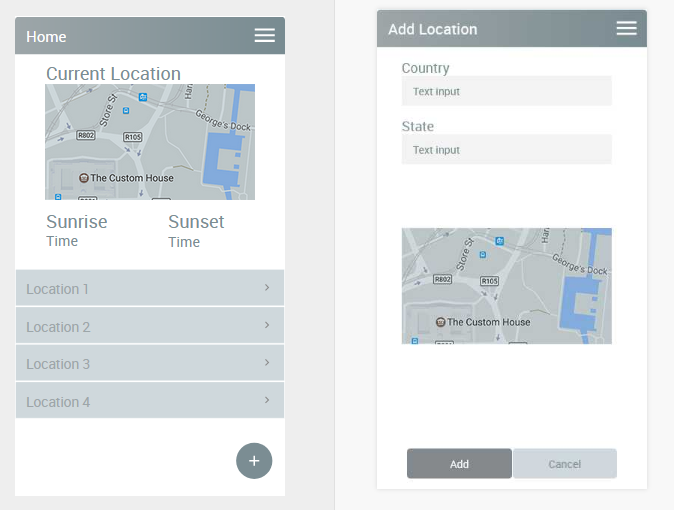
\includegraphics[scale=0.8]{images/screen1.png}
    \caption{The home and add location screens}
\end{figure}

\pagebreak

\begin{figure}[h]
    \centering
    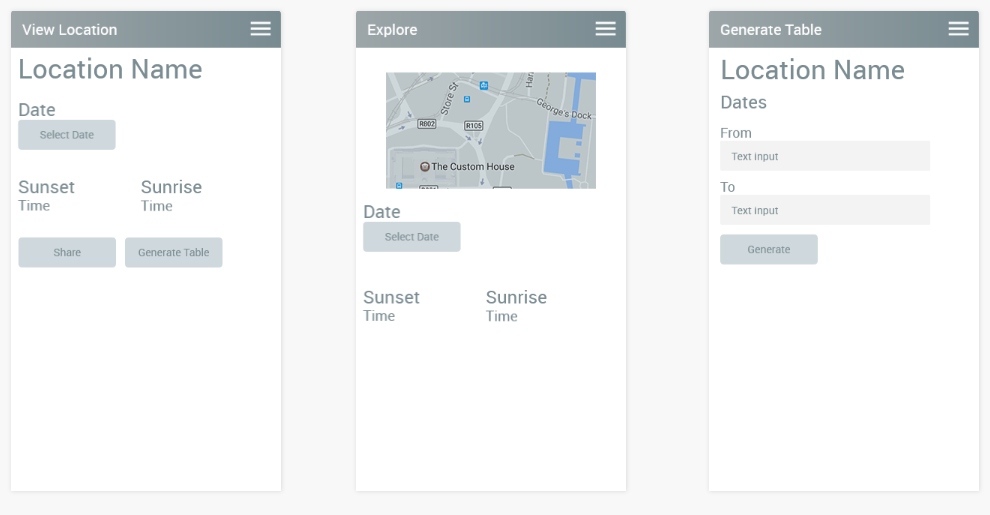
\includegraphics[scale=0.55]{images/screen2.png}
    \caption{The view location, explore, and generate table screens}
\end{figure}

In the above screens I use the following design patterns:

\subsection*{Structured Format}
Whenever the user enters a date (eg. in the explore or view location screens) we require
a proper date format to ensure that we are able to work with it to get the output which
the user expects. This is achieved through a button that opens a calendar interface for
the user. This is important because when we are calculating the sunrise/sunset for a given
location, the code that operates in the background needs structured data so it can properly
process it, which then allows for it to do the necessary calculations.

\subsection*{Input Prompt}
There is a lot of data that the user needs to be able to put into the application to get
information out. Beccause of this, there are many input prompts throughout the application.
The biggest example of this is when the user wishes to add a location to their collection
of locations. When they tap the "+" button on the home screen of the application, they
are taken to an input prompt which asks for their country and state that they want to add
to the application. Once they are done, they are able to either confirm or cancel their
entry with the buttons at the bottom of the screen.

\subsection*{Continuous Scrolling}
On the home screen of the application is a scrolling list of locations that they have saved
to their collection which they can select from. This list can be of an indefinite length,
purely based off how many locations that the user has saved.

\bigskip

The above patterns can be found at:
\begin{itemize}
    \item http://ui-patterns.com/patterns/StructuredFormat
    \item http://ui-patterns.com/patterns/InputPrompt
    \item http://ui-patterns.com/patterns/ContinuousScrolling
\end{itemize}

\section*{Part 2}
The wireflow for the application is as follows:
\begin{figure}[h]
    \centering
    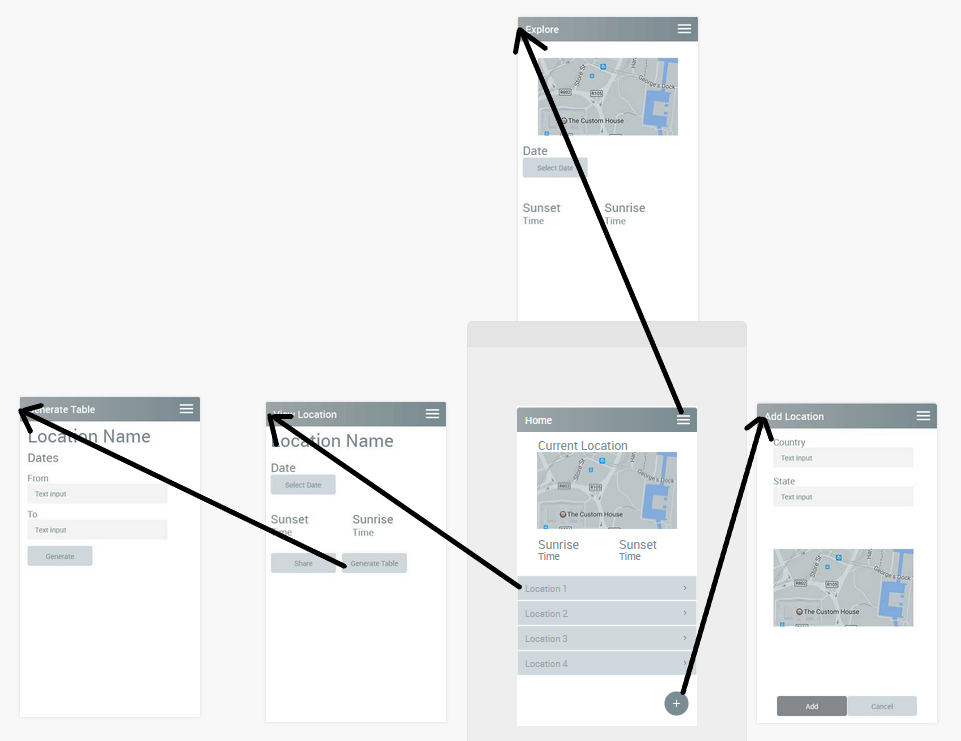
\includegraphics[scale=0.5]{images/wireflow.png}
    \caption{Application wireflow}
\end{figure}

The shortest paths are all just a single tap from the home screen, being the path from
the home screen to the add location, explore, and view location screens. The longest path
then is to the generate table screen which takes two taps from the home screen, to the
location screen, and then finally the generate table screen.

\bigskip

After discussing this design with a friend we came to the following conclusions:
\begin{itemize}
    \item The amount of taps to get to certain screens is low and acceptable
    \item It is not entirely clear how to access the explore page
    \item The home screen might be a bit too cluttered with content
\end{itemize}

\end{document}
